\documentclass{article}
\usepackage{amsfonts} % For open face letters
\usepackage{amsmath} % For align*
\usepackage{float} % For the [H] option on figures
\usepackage{graphicx} % For images
\usepackage{siunitx} % For units
\graphicspath{{./images/}}

\renewcommand{\vec}[1]{\boldsymbol{\mathbf{#1}}}
\newcommand{\dvec}[1]{\dot{\vec{#1}}}
\newcommand{\ddvec}[1]{\ddot{\vec{#1}}}
\newcommand{\uvec}[1]{\hat{\vec{#1}}}

\newcommand{\ke}{\frac{1}{4 \pi \epsilon_0}}

\def\rcurs{{\mbox{$\resizebox{.09in}{.08in}{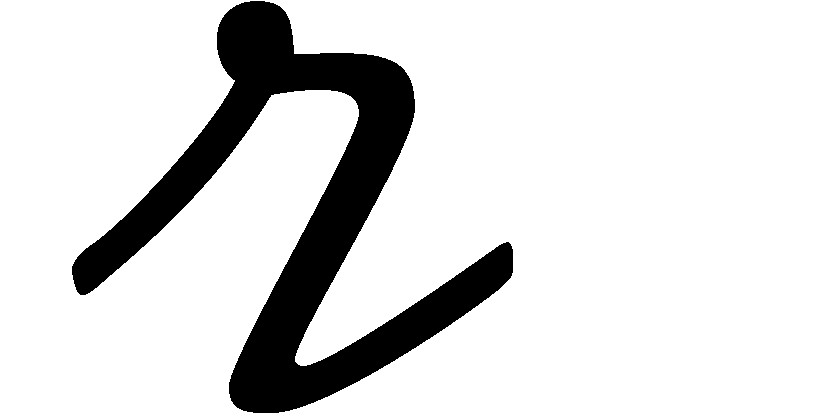
\includegraphics[trim= 1em 0 14em 0,clip]{ScriptR}}$}}}
\def\brcurs{{\mbox{$\resizebox{.09in}{.08in}{
\includegraphics[trim= 1em 0 14em 0,clip]{BoldR}}$}}}
\def\hrcurs{{\mbox{$\hat \brcurs$}}}

\title{Introduction to Electrodynamics by David J. Griffiths Notes}
\author{Chris Doble}
\date{December 2023}

\begin{document}

\maketitle

\tableofcontents

\section{Vector Algebra}

\setcounter{subsection}{5}
\subsection{The Theory of Vector Fields}

\subsubsection{The Helmholtz Theorem}

\begin{itemize}
  \item The \textbf{Helmholtz theorem} states that a vector field $\vec{F}$ is uniquely determined if you're given its divergence $\nabla \cdot \vec{F}$, curl $\nabla \times \vec{F}$, and sufficient boundary conditions.
\end{itemize}

\subsubsection{Potentials}

\begin{itemize}
  \item If the curl of a vector field vanishes everywhere, then it can be expressed as the gradient of a \textbf{scalar potential} \[\nabla \times \vec{F} = \vec{0} \Leftrightarrow \vec{F} = -\nabla V.\]

  \item If the divergence of a vector field vanishes everywhere, then it can be expressed as the curl of a \textbf{vector potential} \[\nabla \cdot \vec{F} = 0 \Leftrightarrow \vec{F} = \nabla \times \vec{A}.\]
\end{itemize}

\section{Electrostatics}

\subsection{The Electric Field}

\setcounter{subsubsection}{1}
\subsubsection{Coulomb's Law}

\begin{itemize}
  \item \textbf{Couloumb's law} gives the force between two point charges $q$ and $Q$ \[\vec{F} = \frac{1}{4 \pi \epsilon_0} \frac{q Q}{\rcurs} \hrcurs\] where \[\epsilon_0 = \qty{8.85e-12}{C^2/(N.m^2)}\] is the \textbf{permittivity of free space} and $\brcurs$ is the separation vector between the two charges.
\end{itemize}

\subsubsection{The Electric Field}

\begin{itemize}
  \item The \textbf{electric field} $\vec{E}$ is a vector field that varies from point to point and gives the force per unit charge that would be exerted on a test charge if placed at a particular point.

  \item For a collection of $n$ source charges $q_i$ at displacements $\brcurs_i$ from a test charge, the electric field is \[\vec{E} = \frac{1}{4 \pi \epsilon_0} \sum_{i = 1}^n \frac{q_i}{\rcurs_i^2} \hrcurs.\]
\end{itemize}

\subsubsection{Continuous Charge Distributions}

\begin{itemize}
  \item Couloumb's law for a continuous charge distribution is \[\vec{E} = \ke \int \frac{1}{\rcurs^2} \hrcurs \,d q.\]
\end{itemize}

\subsection{Divergence and Curl of Electrostatic Fields}

\subsubsection{Field Lines, Flux, and Gauss's Law}

\begin{itemize}
  \item \textbf{Gauss's law} states that the electric field flux through a closed surface is proportional to the amount of charge within that surface \[\oint \vec{E} \cdot d \vec{a} = \frac{1}{\epsilon_0} Q_\text{enc}\] or \[\nabla \cdot \vec{E} = \frac{1}{\epsilon_0} \rho.\]
\end{itemize}

\setcounter{subsubsection}{3}
\subsubsection{The Curl of E}

\begin{itemize}
  \item The curl of an electric field is $\vec{0}$ \[\nabla \times \vec{E} = \vec{0}.\]
\end{itemize}

\subsection{Electric Potential}

\subsubsection{Introduction to Potential}

\begin{itemize}
  \item The \textbf{electric potential} at a point $\vec{r}$ is defined as \[V(\vec{r}) = -\int_\mathcal{O}^{\vec{r}} \vec{E} \cdot d \vec{l}\] where $\mathcal{O}$ is an agreed origin.

  \item The potential difference between two points $\vec{a}$ and $\vec{b}$ is \[V(\vec{b}) - V(\vec{a}) = -\int_{\vec{a}}^{\vec{b}} \vec{E} \cdot d \vec{l}.\]

  \item The electric field and potential are also related by the equation \[\vec{E} = -\nabla V.\]
\end{itemize}

\subsubsection{Comments on Potential}

\begin{itemize}
  \item The choice of origin $\mathcal{O}$ in the definiton of vector potential only affects the absolute potential values, not potential differences. Typically it is chosen to be ``at infinity'' unless the charge distribution itself extends to infinity.

  \item Electric potential obeys the superposition principle.

  \item The units of electric potential is $\unit{N.m/C} = \unit{J/C} = \unit{V}$.
\end{itemize}

\subsubsection{Poisson's Equation and Laplace's Equation}

\begin{itemize}
  \item If \[\nabla \cdot \vec{E} = \frac{\rho}{\epsilon_0}\] and \[\vec{E} = -\nabla V\] then \begin{align*}
          \nabla \cdot (-\nabla V) & = \frac{\rho}{\epsilon_0}   \\
          \nabla^2 V               & = -\frac{\rho}{\epsilon_0}.
        \end{align*} This is known as \textbf{Poisson's equation}. In regions where $\rho = 0$ it reduces to \textbf{Laplace's equation} \[\nabla^2 V = 0.\]
\end{itemize}

\subsubsection{The Potential of a Localized Charge Distribution}

\begin{itemize}
  \item The potential of a continuous charge distribution is \[V(\vec{r}) = \ke \int \frac{\rho(\vec{r}')}{\rcurs} \,d \tau'\] where the reference is point is set to infinity.
\end{itemize}

\subsubsection{Boundary Conditions}

\begin{figure}[H]
  \centering
  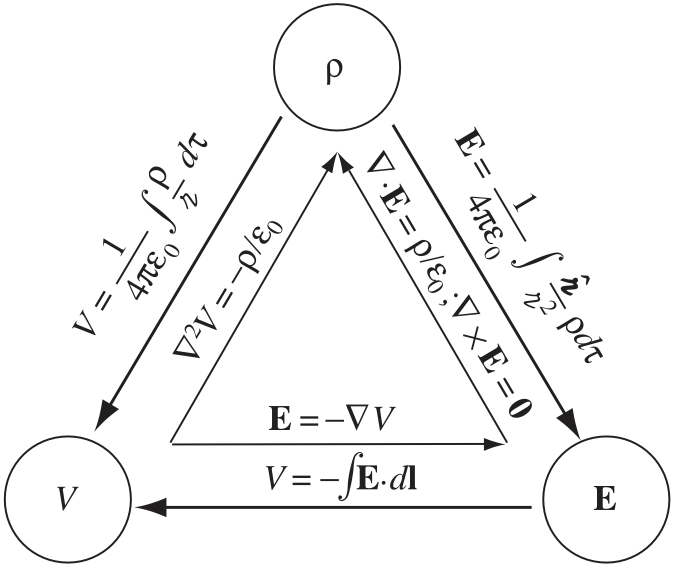
\includegraphics[scale=0.5]{electrostatic-relations}
\end{figure}

\begin{itemize}
  \item The normal component of the electric field is discontinuous by an amount $\sigma / \epsilon_0$ at any boundary, i.e. \[E_\text{above} - E_\text{below} = \frac{\sigma}{\epsilon_0}.\]

  \item The tangential component of the electric field is always continuous at any boundary.

  \item The electric potential is always continuous at any boundary, however because $\vec{E} = -\nabla V$, the gradient of the electric potential inherits the discontinuity at boundaries with surface charge, i.e. \[\nabla V_\text{above} - \nabla V_\text{below} = -\frac{\sigma}{\epsilon_0} \uvec{n}\] or \[\frac{\partial V_\text{above}}{\partial n} - \frac{\partial V_\text{below}}{\partial n} = -\frac{\sigma}{\epsilon_0}\] where \[\frac{\partial V}{\partial n} = \nabla V \cdot \uvec{n}.\]
\end{itemize}

\subsection{Work and Energy in Electrostatics}

\subsubsection{The Work It Takes to Move a Charge}

\begin{itemize}
  \item The work required to move a charge $Q$ from infinity to a point $\vec{r}$ is \[W = Q [V(\vec{r}) - V(\infty)] = Q V(\vec{r}).\] In that sense, the electric potential is the energy per unit charge required to assemble a system of point charges.
\end{itemize}

\subsubsection{The Energy of a Point Charge Distribution}

\begin{itemize}
  \item If you bring a first charge in from infinity you do no work because there are no other charges. If you bring a second charge in from inifnity you do work against the electric field of the first charge. The third does work against the first and second, and so on. Thus the total work required to assemble a collection of charges is \begin{align*}
          W & = \ke \left( \frac{q_1 q_2}{\rcurs_{1 2}} + \frac{q_1 q_3}{\rcurs_{1 3}} + \ldots + \frac{q_1 q_n}{\rcurs{1 n}} + \frac{q_2 q_3}{\rcurs_{2 3}} + \ldots \right) \\
            & = \ke \sum_{i = 1}^n \sum_{j > i}^n \frac{q_i q_j}{\rcurs_{i j}}
        \end{align*} or if we count each pair of charges twice and divide by two \[W = \frac{1}{8 \pi \epsilon_0} \sum_{i = 1}^n \sum_{j \ne i}^n \frac{q_i q_j}{\rcurs_{i j}}.\] If we pull $q_i$ out the front we get \[W = \frac{1}{2} \sum_{i = 1}^n q_i \left( \sum_{j \ne i}^n \ke \frac{q_j}{\rcurs{i j}} \right) = \frac{1}{2} \sum_{i = 1}^n q_i V(\vec{r}_i).\]
\end{itemize}

\subsubsection{The Energy of a Continuous Charge Distribution}

\begin{itemize}
  \item For a volume charge density $\rho$ the work to assemble a continuous charge distribution is \[W = \frac{1}{2} \int \rho V \,d \tau\] or equivalently \[W = \frac{\epsilon_0}{2} \int E^2 \,d \tau\] where the integral is taken over all space.
\end{itemize}

\subsubsection{Comments on Electrostatic Energy}

\begin{itemize}
  \item The energy of an electrostatic field does not obey the superposition principle.
\end{itemize}

\subsection{Conductors}

\subsubsection{Basic Properties}

\begin{itemize}
  \item $\vec{E} = \vec{0}$ inside a conductor because any net electric field causes charges to move, resulting in an induced charge that cancels the electric field.

  \item $\rho = 0$ inside a conductor. By Gauss's law, if $\vec{E} = \vec{0}$ then $\rho$ must also be $0$.

  \item Any net charge resides on the surface of a conductor.

  \item A conductor is an equipotential, i.e. the electric potential is the same everywhere in the conductor.

  \item $\vec{E}$ is perpendicular to the surface of the conductor. If there was a tangential component, charge would move to cancel it.
\end{itemize}

\subsubsection{Induced Charges}

\begin{itemize}
  \item If you hold a charge near an uncharged conductor, the two will attract one another. This is because the external charge causes charges within the conductor to move in order to cancel its magnetic field — like charges are repelled and unlike charges are attracted. This results in unlike charges being closer to the external charge and like charges being further away, resulting in a net attraction.

  \item If you place a charge in a cavity within a conductor, a charge will be induced on the inner surface of the conductor to negate the charge's field within the conductor. If you apply Gauss's law to a Gassian surface that contains the inner charge and inner surface but not the outer surface, the enclosed charge must be $0$. Thus there must be an induced charge of $q$ on the outer surface which communicates the presence of the inner charge to the outside world.

  \item If a cavity within a conductor contains no charge, $\vec{E} = \vec{0}$ within the cavity.
\end{itemize}

\subsubsection{Surface Charge and Force on a Conductor}

\begin{itemize}
  \item Because the field inside a conductor is zero, the boundary condition $E_\text{above} - E_\text{below} = \sigma / \epsilon_0$ requires that the field immediately outside the conductor is \[\vec{E} = \frac{\sigma}{\epsilon_0} \uvec{n}.\] In terms of potential this is \[\sigma = -\epsilon_0 \frac{\partial V}{\partial n}.\]

  \item In the presence of an electric field, a surface charge will experience a force per unit area \[\vec{f} = \sigma \vec{E}_\text{average} = \frac{1}{2} \sigma (\vec{E}_\text{above} + \vec{E}_\text{below}).\] This applies to any surface charge, however for a conductor $\vec{E}_\text{below} = \vec{0}$ so \[\vec{f} = \frac{1}{2} \sigma \vec{E}_\text{above} = \frac{\sigma^2}{2 \epsilon_0} \uvec{n}.\] Notice that this is independent of the sign of $\sigma$. This results in an outward \textbf{electrostatic pressure} on the surface \[P = \frac{\epsilon_0}{2} E^2\] tending to draw the conductor into the field.
\end{itemize}

\subsubsection{Capacitors}

\begin{itemize}
  \item If you have two conductors and place a charge of $+Q$ on one and $-Q$ on the other, an electric field will be induced between them. By Couloumb's law the electric field is proportional to the charge so doubling the charge doubles the electric field and thus the electric potential. The constant of proportionality between the charge and the potential difference between the condutors is called their \textbf{capacitance} \[C = \frac{Q}{V}\] the unit of which is \textbf{farads} ($\unit{F}$).

  \item The work required to fully charge a capacitor to potential difference $V$ is \[W = \frac{1}{2} C V^2.\]
\end{itemize}

\end{document}